%   PACKAGES AND CUSTOMIzATIONS  %%%%%%%%%%%%%%%%%%%%%%%%
\documentclass[12pt]{article}
\usepackage{amsmath}
\usepackage{amssymb}
\usepackage{amsthm}
\usepackage[pdfborder={0 0 0}]{hyperref}
\usepackage{graphicx}
\usepackage{caption}
\usepackage{wrapfig}
\usepackage{enumitem}
\setlist[enumerate]{itemsep=0mm}
\usepackage{multirow}
\usepackage{lscape}
\usepackage{caption}
\usepackage{subcaption}
\usepackage{float}
\usepackage{hyperref}
\usepackage{tabularx}
\usepackage{rotating}
\captionsetup[subfigure]{position=top, labelfont=bf,textfont=normalfont,singlelinecheck=off,justification=raggedright}
\renewcommand{\vector}[1]{\mathbf{#1}}
\usepackage{adjustbox}
\usepackage{bm}


\newcommand{\transectAbb}{Data for each glacier are divided into lower hourglass (LH), lower circle (LC), lower midline (LM), upper hourglass (UH), upper circle (UC), upper midline (UM), and upper transect (UT).}
\newcommand{\params}{Topographic parameters are distance from centreline ($d_C$), elevation ($z$), aspect ($\alpha$), slope ($m$), northness ($N$), curvature ($\kappa$), and Sx. }
\newcommand{\boxplot}{Within each box, the mean is shown as a circle, the median as a horizontal line, the interquartile range (IQR) as a coloured box, two times the IQR as dashed lines beyond the box, and outliers as single points. }
\newcommand{\boxMatlab}{Red line indicates median, blue box shows first quantiles, bars indicate minimum and maximum values (excluding outliers), and red crosses show outliers, which are defined as being outside of the range of 1.5 times the quartiles (approximately $\pm2.7\sigma$). }
\newcommand{\topomap}{Arrows indicate glacier flow direction and black dots show snow depth sampling locations. }
\newcommand{\swedots}{Observed SWE values are overlain on the maps. }


\begin{document}

\section{Transferability}
\label{sec:transferability}

To determine the spatial transferability of LR coefficients, the coefficients from each glacier are used to estimate WSMB on the remaining glaciers. All collected data is then used to generate LR coefficients, which are applied to the study glaciers to estimate WSMB. 


\subsection{Results}

There are considerable differences in the spatial pattern and mean estimated WSMB found using transferred regression coefficients (Figure \ref{fig:MapTransferabilityGlaciersMean}). The spatial patterns found using the Glacier 2 and Glacier 13 coefficients reflect the dominance of elevation within the regression. The uniform distributions found using Glacier 4 coefficients reflect the low regression coefficient values for the topographic parameters on Glacier 4. 

The mean estimated WSMB differs considerably when the various LR coefficients are used. Glacier 4 coefficients result in the highest mean WSMB values because the mean value is approximately equal to the mean of the observed values on Glacier 4, which are higher than that of Glaciers 2 and 13. The range of mean WSMB between different coefficients is especially large for Glacier 4 (0.34 m w.e.).

The range-scale accumulation gradient (Glacier 4 highest accumulation, Glacier 13 lowest accumulation) is not present when using transferred coefficients. Glacier 4 coefficients result in an almost uniform snow distribution on all glaciers. Coefficients from Glaciers 2 and 13 result in Glacier 13 having the highest WSMB. For Glaciers 4 and 2, transferring coefficients decreases the mean WSMB and for Glacier 13, using transferred coefficients increases the mean WSMB. When using all the data to estimate a LR, the mean WSMB and spatial pattern of SWE on each glacier is similar to when Glacier 13 coefficients are used, but the larger LR intercept value results in a higher mean WSMB. 

The WSMB is largely determined by the intercept of the LR used and the magnitude of the elevation regression coefficient (Table \ref{tab:TransferabilityElevCoeffIntercept}) because all other regressors have small coefficients. Therefore, estimating WSMB in the Donjek Range from transferred coefficients is especially sensitive to LR intercept value and magnitude of the elevation regression coefficient.

\pagebreak
\begin{figure}[H]
	\centering
	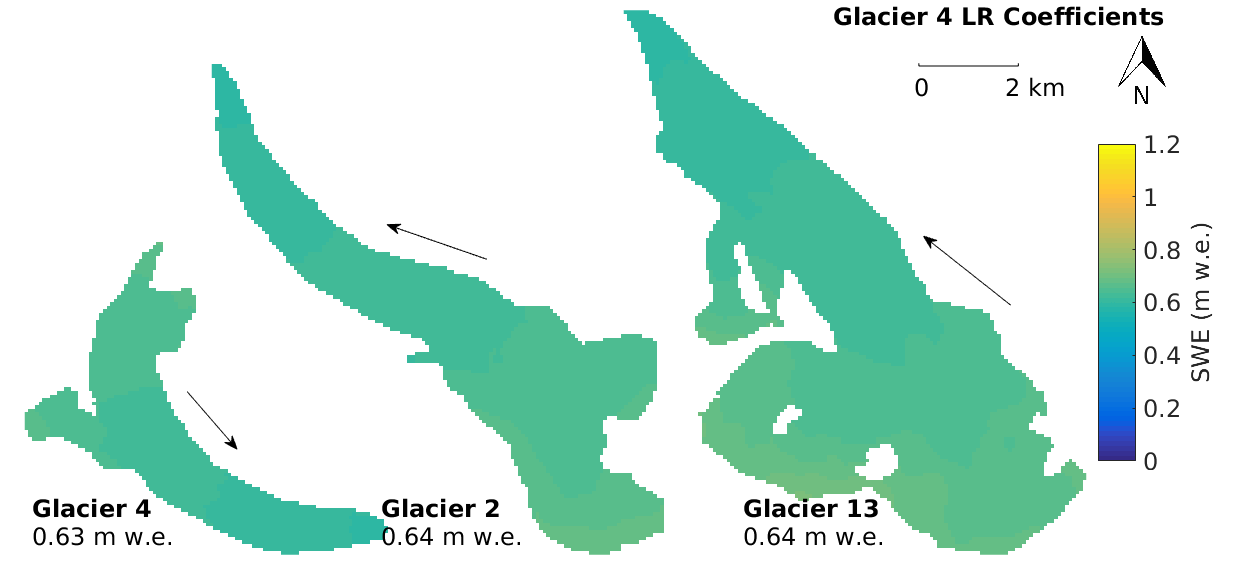
\includegraphics[width =0.9\textwidth]{MapTransferabilityG4Coeffs.png}\\
	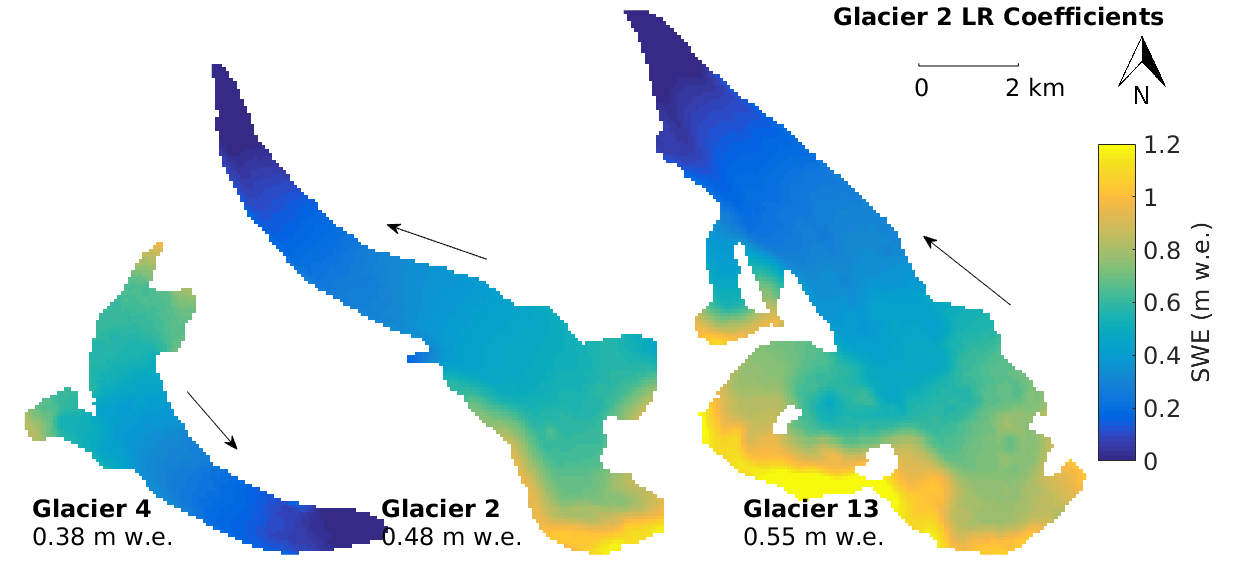
\includegraphics[width =0.9\textwidth]{MapTransferabilityG2Coeffs.png}\\
	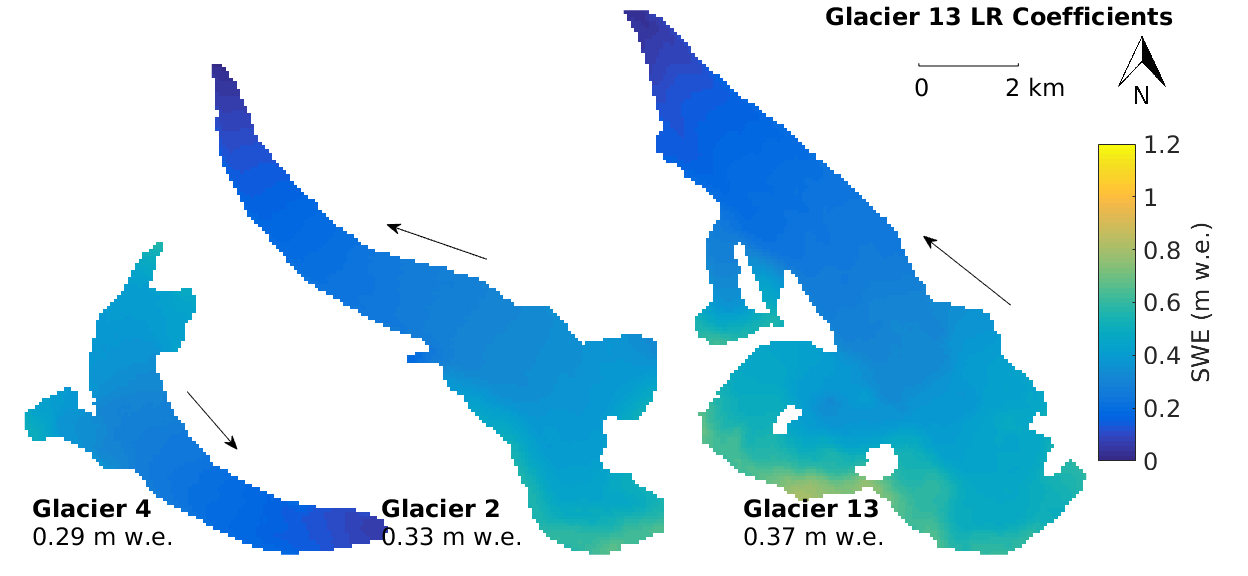
\includegraphics[width =0.9\textwidth]{MapTransferabilityG13Coeffs.png}\\
	\caption{Transfer of LR coefficients to estimate distributed winter surface mass balance (WSMB) on study glaciers. WSMB found using Glacier 4 (top), Glacier 2 (middle) and Glacier 13 (bottom) regression coefficients. The mean SWE from all density interpolation options is shown. Arrows indicate glacier flow direction.}
	\label{fig:MapTransferabilityGlaciersMean}
\end{figure}

\begin{figure}[H]
	\centering
	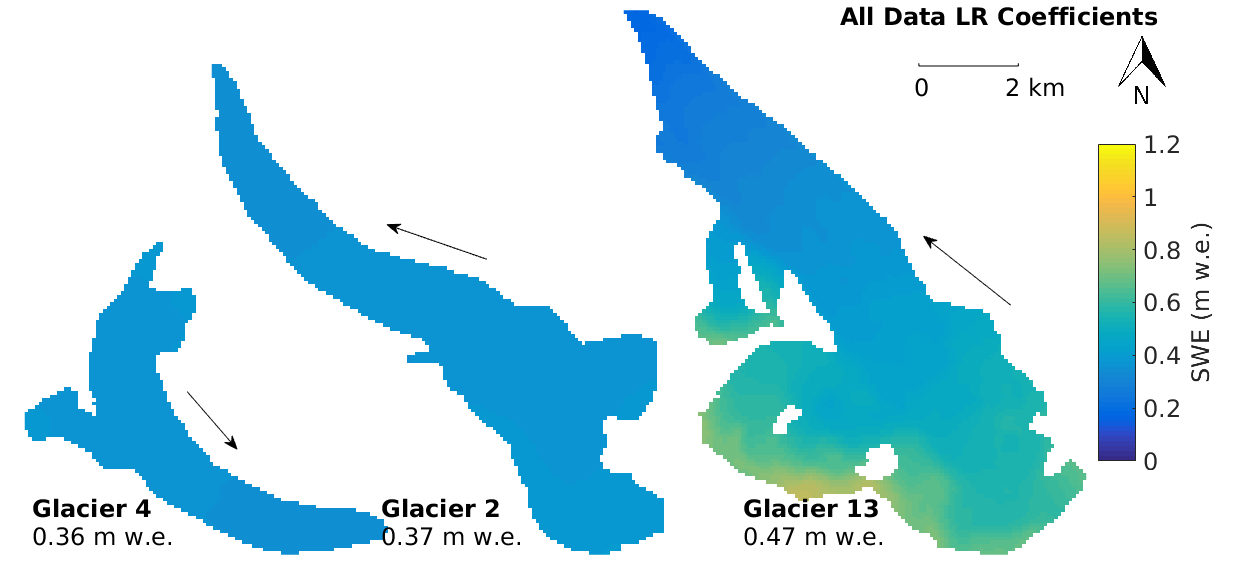
\includegraphics[width =0.9\textwidth]{MapTransferabilityComboCoeffs.png}\\
	\caption{Transfer of LR coefficients to estimate distributed winter surface mass balance (WSMB) on study glaciers. WSMB found using coefficients determined from all available SWE observations. The mean SWE from all density interpolation options is shown. Arrows indicate glacier flow direction.}
	\label{fig:MapTransferabilityComboMean}
\end{figure}

\begin{table}[h]
\centering
\caption{Elevation regression coefficients and intercepts used in linear regression transferability. The mean RMSE for all glaciers is also shown.}
\label{tab:TransferabilityElevCoeffIntercept}
\begin{tabular}{ccccc}
 & \textbf{\begin{tabular}[c]{@{}c@{}}Glacier 4\\ Coefficients\end{tabular}} & \textbf{\begin{tabular}[c]{@{}c@{}}Glacier 2\\ Coefficients\end{tabular}} & \textbf{\begin{tabular}[c]{@{}c@{}}Glacier 13 \\ Coefficients\end{tabular}} & \textbf{\begin{tabular}[c]{@{}c@{}}All Data \\ Coefficients\end{tabular}} \\ \hline \hline
\begin{tabular}[c]{@{}c@{}}Elevation \\ Regression\\ Coefficient\end{tabular} & 0.0082 & 0.1084 & 0.0510 & 0.0523 \\ \hline
\begin{tabular}[c]{@{}c@{}}Intercept\\ (m w.e)\end{tabular} & 0.6217 & 0.2497 & 0.2247 & 0.3435 \\ \hline
\begin{tabular}[c]{@{}c@{}}Mean RMSE\\ (m w.e.)\end{tabular} & 0.3066 & 0.2065 & 0.2142 & 0.1994
\end{tabular}
\end{table}


The RMSE of estimated WSMB found using transferred coefficients is larger for all glaciers then when using glacier specific coefficients (Figure \ref{fig:TransferabilityRMSE}). Glacier 4 coefficients introduce a large RMSE for Glaciers 2 and 13, while all other coefficient sets result in large RMSE on Glacier 4. Glaciers 2 and 13 have relatively small changes in RMSE when coefficients from Glacier 2, Glacier 13 or all data coefficients are used. Interestingly, the lowest average RMSE for all glaciers occurs when all data coefficients are used (Table \ref{tab:TransferabilityElevCoeffIntercept}). Therefore, if transfer of coefficients is needed, using all the data to generate LR coefficients will result in the lowest error with observed values.  



\begin{figure}[H]
	\centering
	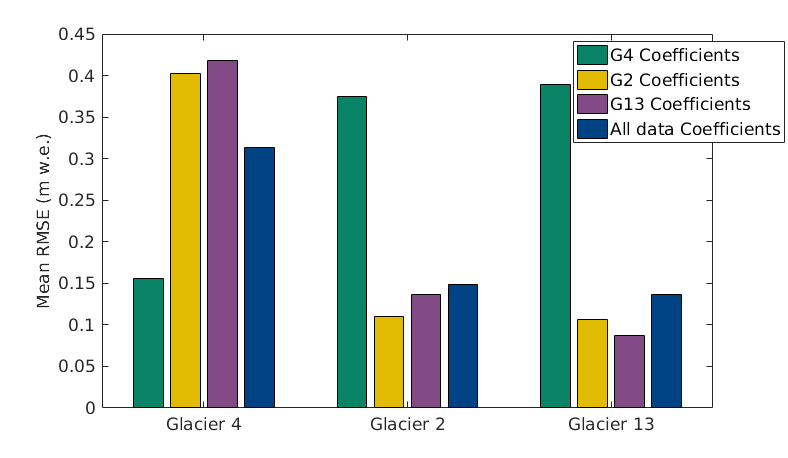
\includegraphics[width =0.8\textwidth]{TransferabilityRMSE.png}\\
	\caption{Root mean squred error (RMSE) at sampling locations when LR coefficients are transfered between glaciers. The mean RMSE from all density interpolation options is shown.}
	\label{fig:TransferabilityRMSE}
\end{figure}

%%%%%%%%%%%%%%%%%%%%%

\end{document} 